\section{Exponenciální funkce}
\begin{definition}
    Nechť $a\in \mathbb R^+ \smallsetminus \left \{ 1 \right \}. $ Pak funkci $f:y=a^x$
    nazýváme \textbf{exponenciální funkcí} o základu $a$. Funkci $f:y=e^x$ pak
    nazveme \textbf{přirozenou exponenciální funkcí}.
\end{definition}

\begin{figure}[ht!]
  \centering
  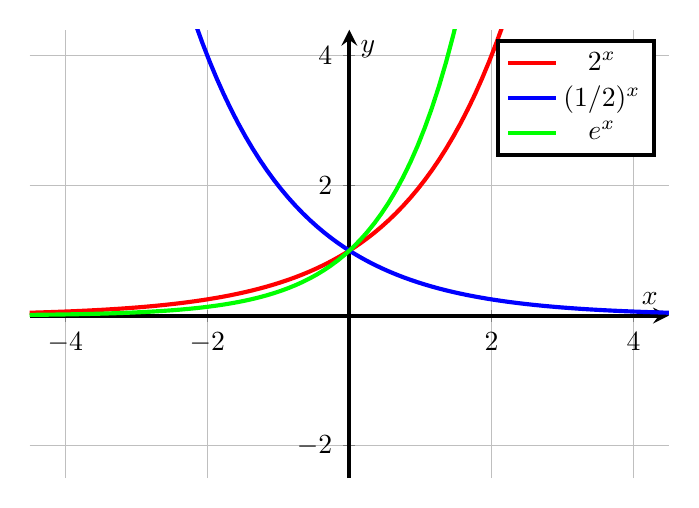
\begin{tikzpicture}
    \begin{axis}[
        axis lines = middle,
        xlabel = \(x\),
        ylabel = {\(y\)},
        line width=1.5pt,
        width=.8\textwidth,
        height=.6\textwidth,
        ymin=-2.5,
        ymax=4.4,
        xmin=-4.5,
        xmax=4.5,
        grid
    ]
    %Below the red parabola is defined
    \addplot [
        domain=-5:5,
        samples=100,
        color=red
    ]
    {2^x};
    \addlegendentry{\(2^x\)}

    \addplot [
        domain=-5:5,
        samples=100,
        color=blue
        ]
        {0.5^x};
    \addlegendentry{\((1/2)^x\)}

    \addplot [
        domain=-5:5,
        samples=100,
        color=green
        ]
        {e^x};
    \addlegendentry{\(e^x\)}

    \end{axis}
    \end{tikzpicture}
  \caption{Grafy některých exponenciálních funkcí}
\end{figure}

\begin{veta}
    Vlastnosti exponenciálních funkcí $y= a^x$, kde $a$ je přirozené číslo:
    \begin{enumerate}[$i.$]
        \item $D(f)= \mathbb R$, $H(f)= \mathbb R^+$.
       	\item Graf každé exponenciální funkce prochází bodem $[0,1].$
        \item Není ani sudá, ani lichá.
        \item Je zdola omezená.
        \item Pro $a >1$ je rostoucí, pro $a<1$ je klesající.
        \item Nemá extrémy a není periodická.
    \end{enumerate}
\end{veta}

\begin{definition}
    (Ne)rovnice s neznámou v exponentu se nazývá \textbf{exponenciální (ne)rovnice}.
\end{definition}

\begin{veta}
    $\forall a \in \mathbb R^+ \smallsetminus \left \{ 1 \right \}, \forall x_1, x_2
    \in \mathbb R: a^{x_1}=a^{x_2}\iff x_1=x_2.$
\end{veta}

\begin{proof}
    Plyne z toho, že exponenciální funkce je prostá.
\end{proof}

\begin{priklad}
Určete, pro která $b\in \mathbb R\smallsetminus\left \{ 1 \right \} $ je $f:y=\left ( \frac{b}{b-1} \right )^x $
rostoucí a pro která klesající.
\end{priklad}

\begin{reseni}
Je rostoucí, pokud základ je větší než 1 a klesající, pokud základ je menší než 1.
Řešíme tedy
\begin{align*}
\frac{b}{b-1}>1, & & \textrm{resp.} & & \frac{b}{b-1}<1.
\end{align*}
\end{reseni}
